\documentclass[10pt]{article}
\usepackage{icmlko}

\icmlmeta{IP 파운데이션 월드모델}{198}{사이에 있을 줄 알았는데 끝에 있었다}{노트 197이 ``혼자냐 풀링이냐를 이분으로 고르는데 진짜 답은 그 사이에 있을 것''으로 닫았다. 반대다 --- 유보는 날카로울수록 좋고, 안쪽은 그것을 전혀 못 본다}

\begin{document}

\twocolumn[
\icmlheader

\begin{abstract}
노트 197이 도메인마다 ``혼자냐 풀링이냐''를 안쪽에서 골라 $+$0.3822 를
$+$0.3955 로 올리고, ``이분 대신 축소 비율로 섞으면 더 나을 것''을 남겼다.
섞었다 --- $\beta_d = \lambda_d \beta_{\text{혼자}} + (1-\lambda_d)
\beta_{\text{풀링}}$ 이고 $\lambda_d = \sigma(k \cdot \text{안쪽격차}_d)$ 로
손잡이가 $k$ 하나다. \textbf{두 가지가 나왔고 둘 다 예상과 다르다.}
\textbf{① 유보는 $k$ 에 완벽히 단조다}(스피어만 $+$1.000) --- $k{=}0$ 의
$+$0.3852 에서 $k{=}200$ 의 $+$0.3998 까지 계속 오른다. $k{=}200$ 이면
$\lambda$ 가 사실상 0 아니면 1 이다. \textbf{섞는 것이 아니라 날카로운 쪽이
낫다} --- 노트 197의 닫는 가설이 반증됐다. \textbf{② 안쪽은 그것을 전혀
못 본다.} 안쪽 $k$ 곡선의 폭이 0.0104 이고 유보와의 상관이
\textbf{$+$0.036} 이다 --- 사실상 0. 안쪽은 $k{=}20$ 을 고르는데 그 점의
유보가 $+$0.3886 으로 노트 197의 이분($+$0.3955)보다 낮다. \textbf{규약이
막았다} --- 봉우리 0.226 · 단조 0.036 으로 둘 다 문턱 아래다.
\textbf{네 번째로 옳게 막았다}(노트 190 · 193 에서 셋, 여기서 하나). 그리고
이번 것은 \emph{왜} 막아야 했는지가 제일 선명하다 --- 안쪽 신호가 약한 게
아니라 \textbf{유보와 무관}하다($+$0.036). \textbf{채택은 노트 197의 이분
규칙 그대로다}($+$0.3955). 남은 것을 정직하게 적는다: 유보에서 제일 좋은
점은 $k{=}200$ 의 $+$0.3998 이고, 거기서 세계애니가 $\lambda{=}0.94$ ·
애니가 $0.66$ 으로 \emph{부분} 혼자다 --- \textbf{완전한 이분보다 낫지만
안쪽에서 그 점을 못 찾는다.}
\end{abstract}
]

\begin{figure*}[t]
\centering
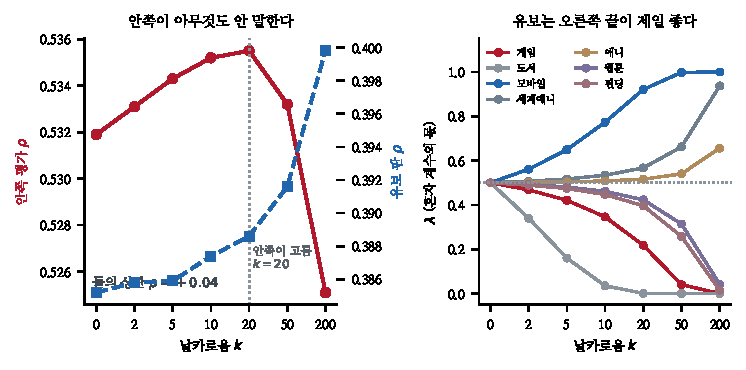
\includegraphics[width=.74\textwidth]{figs/sharp.pdf}
\caption{왼쪽 --- 안쪽이 아무것도 안 말한다. 오른쪽 --- 유보는 오른쪽 끝이
제일 좋다.}
\end{figure*}

\section{유보는 날카로울수록 좋다}

\begin{table}[t]
\centering\tsize
\caption{$\lambda_d = \sigma(k\cdot\text{안쪽격차}_d)$.}
\begin{tabular}{rrr}
\toprule
$k$ & 안쪽 평가 & 유보 판 \\
\midrule
0 (반반) & .5319 & .3852 \\
5 & .5343 & .3859 \\
\textbf{20} & \textbf{.5355} & .3886 \\
50 & .5332 & .3916 \\
\textbf{200} & .5251 & \textbf{.3998} \\
\midrule
\multicolumn{2}{l}{유보의 $k$ 단조성} & $\rho{=}+1.000$ \\
\multicolumn{2}{l}{안쪽 $\leftrightarrow$ 유보} & $\rho{=}+0.036$ \\
\bottomrule
\end{tabular}
\end{table}

\claimx{\textbf{유보가 완벽히 단조다}($\rho{=}+1.000$). $k$ 를 키울수록 계속
좋아지고 $k{=}200$ 이면 $\lambda$ 가 사실상 0 아니면 1 이다.}{\textbf{노트
197의 닫는 가설이 반증됐다} --- ``진짜 답은 그 사이에 있을 것''이라고
적었는데 끝에 있다. 이 흐름에서 결론 옆에 적은 까닭이 틀린 것이 여덟
번째다.}

\claimx{읽기 하나 --- 안쪽 격차의 \emph{크기}는 못 믿고 \emph{부호}만 믿을
만하다. 격차가 모바일 $+$0.123 · 세계애니 $+$0.014 · 애니 $+$0.003 인데,
크기를 그대로 쓰면($k$ 작음) 세 도메인이 다 반반이 되어 정보가
사라진다.}{$k$ 를 키우면 부호만 남고 크기가 지워진다 --- 그래서 좋아진다.
\textbf{잡음이 크기에 있고 신호가 부호에 있다.}}

\section{안쪽은 그것을 못 본다}

\claimx{\textbf{안쪽과 유보의 상관이 $+$0.036 이다.} 약한 게 아니라
\emph{무관}하다. 안쪽 폭이 0.0104 로 유보 폭 0.0146 과 비슷한데 방향이
안 맞는다.}{안쪽 격차를 안쪽 평가 구간에서 재고 같은 구간에서 $k$ 를
고르는 것이라 순환이 있다 --- \textbf{$k$ 를 키우면 그 순환이 커져 안쪽이
오히려 나빠진다}($k{=}200$ 에서 0.5251). 유보에서는 반대다.}

\claimx{\textbf{규약이 막았다} --- 봉우리 0.226 · 단조 0.036. 막힌 뒤
채택은 노트 197의 이분 규칙 그대로($+$0.3955)이고, 안쪽이 고른 $k{=}20$
($+$0.3886)보다 높다.}{\textbf{네 번째로 옳게 막았다.} 노트 190에서 챔피언
조정 하나, 노트 193에서 두 방식, 여기서 하나. \textbf{이번 것은 왜
막아야 했는지가 제일 선명하다} --- 안쪽 신호가 유보와 무관하다는 것을
사후에 확인했다.}

\section{정직하게 남기는 것}

\begin{table}[t]
\centering\tsize
\caption{$k{=}200$ 에서의 $\lambda$ (혼자 계수의 몫).}
\begin{tabular}{lrr}
\toprule
& 안쪽 격차 & $\lambda$ \\
\midrule
모바일 & $+$.123 & 1.00 \\
\textbf{세계애니} & $+$.014 & \textbf{0.94} \\
\textbf{애니} & $+$.003 & \textbf{0.66} \\
웹툰 & $-$.016 & 0.04 \\
펀딩 & $-$.021 & 0.01 \\
게임 & $-$.064 & 0.00 \\
도서 & $-$.332 & 0.00 \\
\bottomrule
\end{tabular}
\end{table}

\claimx{\textbf{유보 최고점은 완전한 이분이 아니다.} 세계애니 0.94 · 애니
0.66 으로 \emph{부분} 혼자이고, 그 점이 $+$0.3998 로 이분($+$0.3955)보다
높다.}{\textbf{그래도 못 가져간다} --- 안쪽이 그 점을 못 찾는다. 노트 195의
``보이지 않는 이득은 못 가져간다''가 여기서 반복된다. 그때는 $+$0.007
이었고 여기는 $+$0.004 다.}

\claimx{\textbf{두 노트가 같은 모양이다.} 노트 195 · 198 둘 다 ``유보에서
더 좋은 점이 있는데 안쪽에서 안 보인다''로 끝난다. 합치면 $+$0.011 을
규약 때문에 못 가져간다.}{그 대가를 치르는 대신 노트 190 · 193 · 198 에서
$-$0.010 · $-$0.011 · $-$0.007 짜리 잘못된 선택 넷을 막았다 ---
\textbf{계산서는 여전히 규약 쪽이 이긴다.}}

\begin{table}[t]
\centering\tsize
\caption{이 갈래의 판.}
\begin{tabular}{lr}
\toprule
완전 분리 & .3445 \\
완전 풀링 & .3822 \\
축소 비율(안쪽이 고름) & .3886 \\
\textbf{이분(노트 197 · 채택)} & \textbf{.3955} \\
(유보 최고점 --- 못 가져감) & .3998 \\
\bottomrule
\end{tabular}
\end{table}

\begin{table}[t]
\centering\tsize
\caption{남은 것.}
\begin{tabular}{ll}
\toprule
\textbf{부호만} & 격차의 크기를 버리고 부호만 쓰면 \\
안쪽 순환 & 격차와 평가를 다른 구간에서 \\
트리 & 이 갈래 전체가 능형만 \\
\bottomrule
\end{tabular}
\end{table}

두 번째 줄이 첫 줄을 고치는 길이다. 지금은 안쪽 격차를 \texttt{IN\_TE} 에서
재고 $k$ 도 \texttt{IN\_TE} 에서 고른다 --- 같은 자료를 두 번 쓰는 순환이라
안쪽 곡선이 뒤집힌다($k$ 가 커질수록 안쪽이 나빠지는데 유보는 좋아진다).
\textbf{학습 구간을 셋으로 잘라 격차는 둘째 토막에서, $k$ 는 셋째 토막에서
재면} 순환이 사라지고 안쪽이 유보를 따라갈 수 있다. \textbf{그러면 $k{=}200$
쪽을 고를 수 있고 $+$0.004 를 되찾는다} --- 다만 토막이 셋이 되면 각각이
작아져 노트 192가 잰 용량 편향이 커진다. \textbf{어느 쪽이 큰지는 재 봐야
안다.}

\end{document}
